\documentclass[sigconf]{acmart}
% ----------------------------------------------------------------------
% ACM Required Metadata
% ----------------------------------------------------------------------
\settopmatter{printacmref=false}
\renewcommand\footnotetextcopyrightpermission[1]{}

%\copyrightyear{2025}
\acmYear{2025}
\setcopyright{rightsretained}
\acmConference[ConfName '25]{Conference Name}{Month DD--DD, 2025}{City, Country}
\acmDOI{10.1145/nnnnnnn.nnnnnnn}
\acmISBN{978-1-4503-XXXX-X/25/05}


% ----------------------------------------------------------------------
% Packages (optional)
% ----------------------------------------------------------------------
\usepackage[most]{tcolorbox}
\tcbset{
  colback=gray!10,
  colframe=gray!50,
  boxrule=0.5pt,
  arc=3mm,
  left=6pt,
  right=6pt,
  top=6pt,
  bottom=6pt,
}
\tcbuselibrary{listings, skins}
\usepackage{amsmath}
\usepackage{float} % table/graph close to paragraph
\usepackage{graphicx}
\usepackage{booktabs}
\usepackage{multirow}
\usepackage{tcolorbox}
\usepackage{listings}
\lstset{
    basicstyle=\ttfamily\small,
    breaklines=true,
    frame=single
}
\lstset{
  breaklines=true,
  breakatwhitespace=true,
}
% \newtcolorbox{promptbox}[2][]{
%   title={#2},
%   colback=white,
%   colframe=black,
%   fonttitle=\bfseries,
%   listing only,
%   listing options={
%       basicstyle=\ttfamily\small,
%       breaklines=true,
%       keywordstyle=\color{blue},    % highlight
%       commentstyle=\color{red},     % highlight
%       columns=fullflexible
%   },
%   #1
% }
\newtcolorbox{promptbox}[2][]{
  enhanced,
  % breakable,             
  title={#2},
  colback=white,
  colframe=black,
  fonttitle=\bfseries,
  listing only,
  listing options={
      basicstyle=\ttfamily\small,
      breaklines=true,      
      breakatwhitespace=true,
      columns=fullflexible
  },
  #1
}

\usepackage{graphicx}

% ----------------------------------------------------------------------
% Title and Authors
% ----------------------------------------------------------------------
\title{\textbf{M.U.S.E.: Multi-agent Symbolic Music Understanding with LLMs}}

\author{Qicheng Jin}
\affiliation{
  \institution{University of Chicago}
  \city{Chicago}
  \country{United States}
}
\author{Chenqi Wang}
\affiliation{
  \institution{University of Chicago}
  \city{Chicago}
  \country{United States}
}
\author{Chenxi Peng}
\affiliation{
  \institution{University of Chicago}
  \city{Chicago}
  \country{United States}
}

\raggedbottom % encourage latex to stretch the text slightly to fill the page properly without leaving a huge gap
% ----------------------------------------------------------------------
% Begin Document
% ----------------------------------------------------------------------
\begin{document}

\begin{abstract}
Symbolic music encodes compositions as discrete events such as pitches, durations, and bar structures, making it suitable for large language models (LLMs) to analyze. Despite their strong performance in natural language processing, LLMs often struggle with music-theoretic reasoning, including key signatures, pitch relationships, and higher-level semantic interpretation. In response to these challenges, we propose M.U.S.E., a multi-agent system designed to handle symbolic music understanding tasks. Using ABC notation, we evaluate both pure LLMs and our multi-agent system on benchmark tasks that convert symbolic music questions into multiple-choice or quantitative formats. These tasks provide objective measures of whether models genuinely interpret symbolic structure rather than relying on surface-level heuristics. The results demonstrate that M.U.S.E. outperforms LLMs alone on syntax understanding and emotion recognition tasks, showing the potential of a multi-agent approach to improving LLMs’ ability to understand symbolic music.
\end{abstract}

\keywords{Symbolic music, agentic AI, ABC notation, reasoning}

\maketitle

% ----------------------------------------------------------------------
% Sections
% ----------------------------------------------------------------------

\section{Introduction}
Symbolic music is a crucial concept in the field of digital audio and music information retrieval. It refers to a data format that records and represents music using "musical score" logic. Common formats of symbolic music are MIDI (.mid), MusicXML (.xml), and ABC (.abc). If we compare a piece of music to a speech, then audio is the recording file of the speech (recording the waveform of the sound), while symbolic music is the transcript of the speech (recording every word, intonation, and pause). It represents musical pieces as a sequence of discrete and abstract events, such as pitch, duration, and time, rather than an audio waveform. This structural representation can allow analysis and manipulation of musical elements like notes, harmony, and rhythm. 

In the context of digital humanities and artificial intelligence, people's interest in understanding symbolic music has risen gradually. This transition reflects that people are not only satisfied by listening to the music at the surface level, but also hope to understand the basic ``grammar'' behind the music production. This pursuit has profound practical significance, especially in the computational music and generative AI areas. Using symbolic music, the researchers can train more complex models, enabling them to compose coherent music, automatically performing complex musical notation, and develop adaptive educational tools that can respond in real time to musicians' performances. In general, understanding symbolic music bridges the gap between human creativity and machine logic, opening up endless possibilities for the creation, analysis, and preservation of music.

The discrete nature of symbolic music, similar to text, allows it to be tokenized and processed by language models. MusicBERT \citep{zengMusicBERTSymbolicMusic2021} is a large-scale pre-trained model for symbolic music understanding. It didn't adopt the pre-training methods from NLP to symbolic music, but designed some methods, like the efficient and universal OctupleMIDI encoding, the effective bar-level masking strategy, and the large-scale symbolic music corpus with more than 1 million music songs. This innovation makes the model perform better in four evaluated symbolic music understanding tasks, including melody completion, accompaniment suggestion, genre classification, and style classification. 

The pre-training corpora of LLMs typically contain large amounts of music-related text and raw symbolic music data, making it possible to apply them to symbolic music understanding tasks \citep{zhouCanLLMsReason2024a}. Previous studies have shown inconsistencies in the performance of LLMs on symbolic music understanding tasks. \citet{maMusicLLMsLearn2024} applied a probing and intervention method to Music LLMs to explore their ability to understand musical concepts. The result shows that these models indeed acquire the concept of pitch and chord root. Some studies also find good performance of LLMs on basic syntax understanding \citep{shinLargeLanguageModels2025}\citep{yuanChatMusicianUnderstandingGenerating2024a}. However, LLMs may struggle significantly with the explicit logical reasoning required for complex composition and analysis. \citet{zhaoABCEvalBenchmarkingLarge2025} create an ABC-based benchmark target to assess the symbolic music understanding and instruction-following capabilities of LLMs. They reveal notable limitations in the high-level understanding capabilities of LLMs. For example, sequence-level tasks such as emotion recognition and genre recognition. \citet{zhouCanLLMsReason2024a} also identify that current LLMs exhibit poor performance in song-level multi-step music reasoning. When addressing complex musical tasks, they fail to leverage learned music knowledge. Based on the previous studies, we can see that there is a huge gap between music knowledge and reasoning. Therefore, how to enhance LLMs' reasoning ability in symbolic music is still an exciting direction worth exploring.

\begin{figure*}[ht]
    \centering
    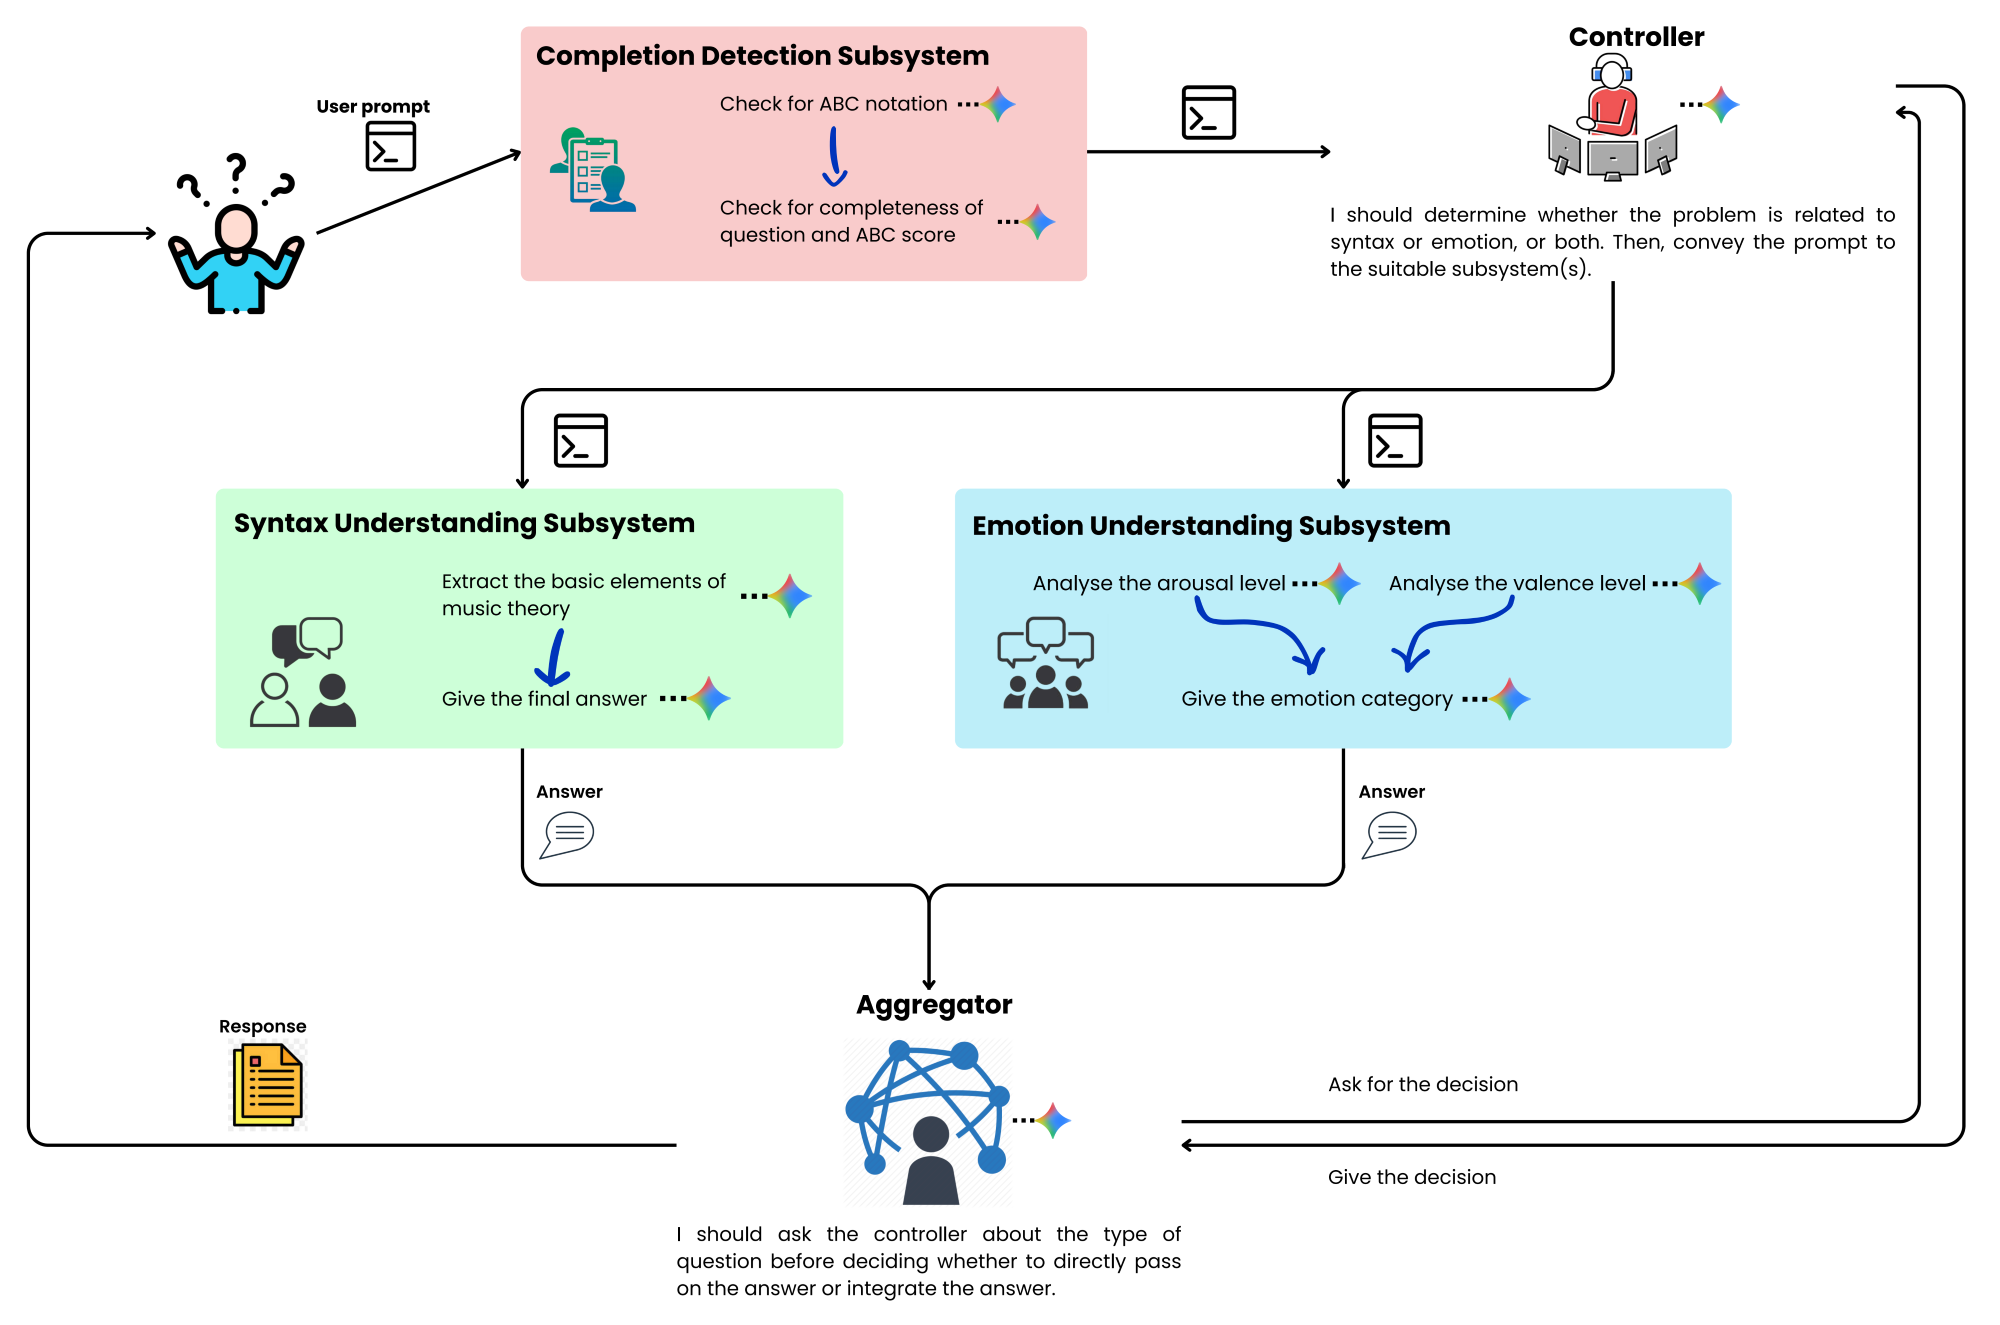
\includegraphics[width=\textwidth]{images/Copy of Agent system_2.png}
    \Description{A system diagram illustrating the framework. On the left, a user input block feeds into an agent block. The agent block connects to a musical score generation module...}
    \caption{The framework of M.U.S.E.: The system receives a user prompt. The Completion Detection Subsystem checks whether the ABC score and the question are complete. If both are valid, the prompt is sent to the Controller Agent, which determines the appropriate subsystem(s) to activate. Two subsystems handle the questions: the syntax understanding subsystem, which answers questions related to music-theory syntax, and the emotion understanding subsystem, which identifies emotional categories. Finally, the Aggregator combines the Controller’s decisions and the output(s) of subsystems to generate the final response for the user.}
    \label{fig:system}
\end{figure*}

On the basis of these LLM capabilities, many researchers have expanded the scope of the LLMs as controllers to orchestrate various domain-specific expert models to solve complex AI tasks, such as HuggingGPT \citep{shenHuggingGPTSolvingAI2023}, AutoGPT, and other modal-specific models \citep{chenVisualGPTDataefficientAdaptation2022}\citep{wuVisualChatGPTTalking2023}\citep{huangAudioGPTUnderstandingGenerating2023}. These successes have inspired us to explore the possibility of designing a system capable of enhancing the high-level understanding capabilities of LLMs in symbolic music, better assisting musicians and music lovers in understanding symbolic music.

Recent advances in agent-based methods have accelerated the development of intelligent music analysis and composition. WeaveMuse \citep{karystinaiosWeaveMuseOpenAgentic2025} is an open intelligent agent system for multimodal music understanding and generation. At its core, it integrates multi-agent collaboration and modular tools to achieve cross-modal interaction between text, symbolic notation, and audio, and supports local and cloud deployment. Similarly, MusicAgent \citep{yuMusicAgentAIAgent2023} is an autonomous intelligent agent for the music domain, powered by LLM, providing an end-to-end automated solution for music processing. It consists of two core components: a toolset covering generation, understanding, and auxiliary tasks; and an autonomous workflow using LLM for task planning, tool selection, and response generation. It also provides plug-in modules for optimizing GPU resource utilization and supports three deployment methods: code invocation, command line, and gradient visualization.

These multi-agent solutions heavily rely on external computational resources or tools and depend on GPU servers for deploying local inference services. Although they may address issues related to diverse data formats and platforms, they cannot leverage the intrinsic musical understanding of LLMs and tend to overuse external processes for music understanding tasks, which may lead to failures in interpreting symbolic music. In sum, the contributions of our paper are as follows:

\begin{figure*}
    \centering
    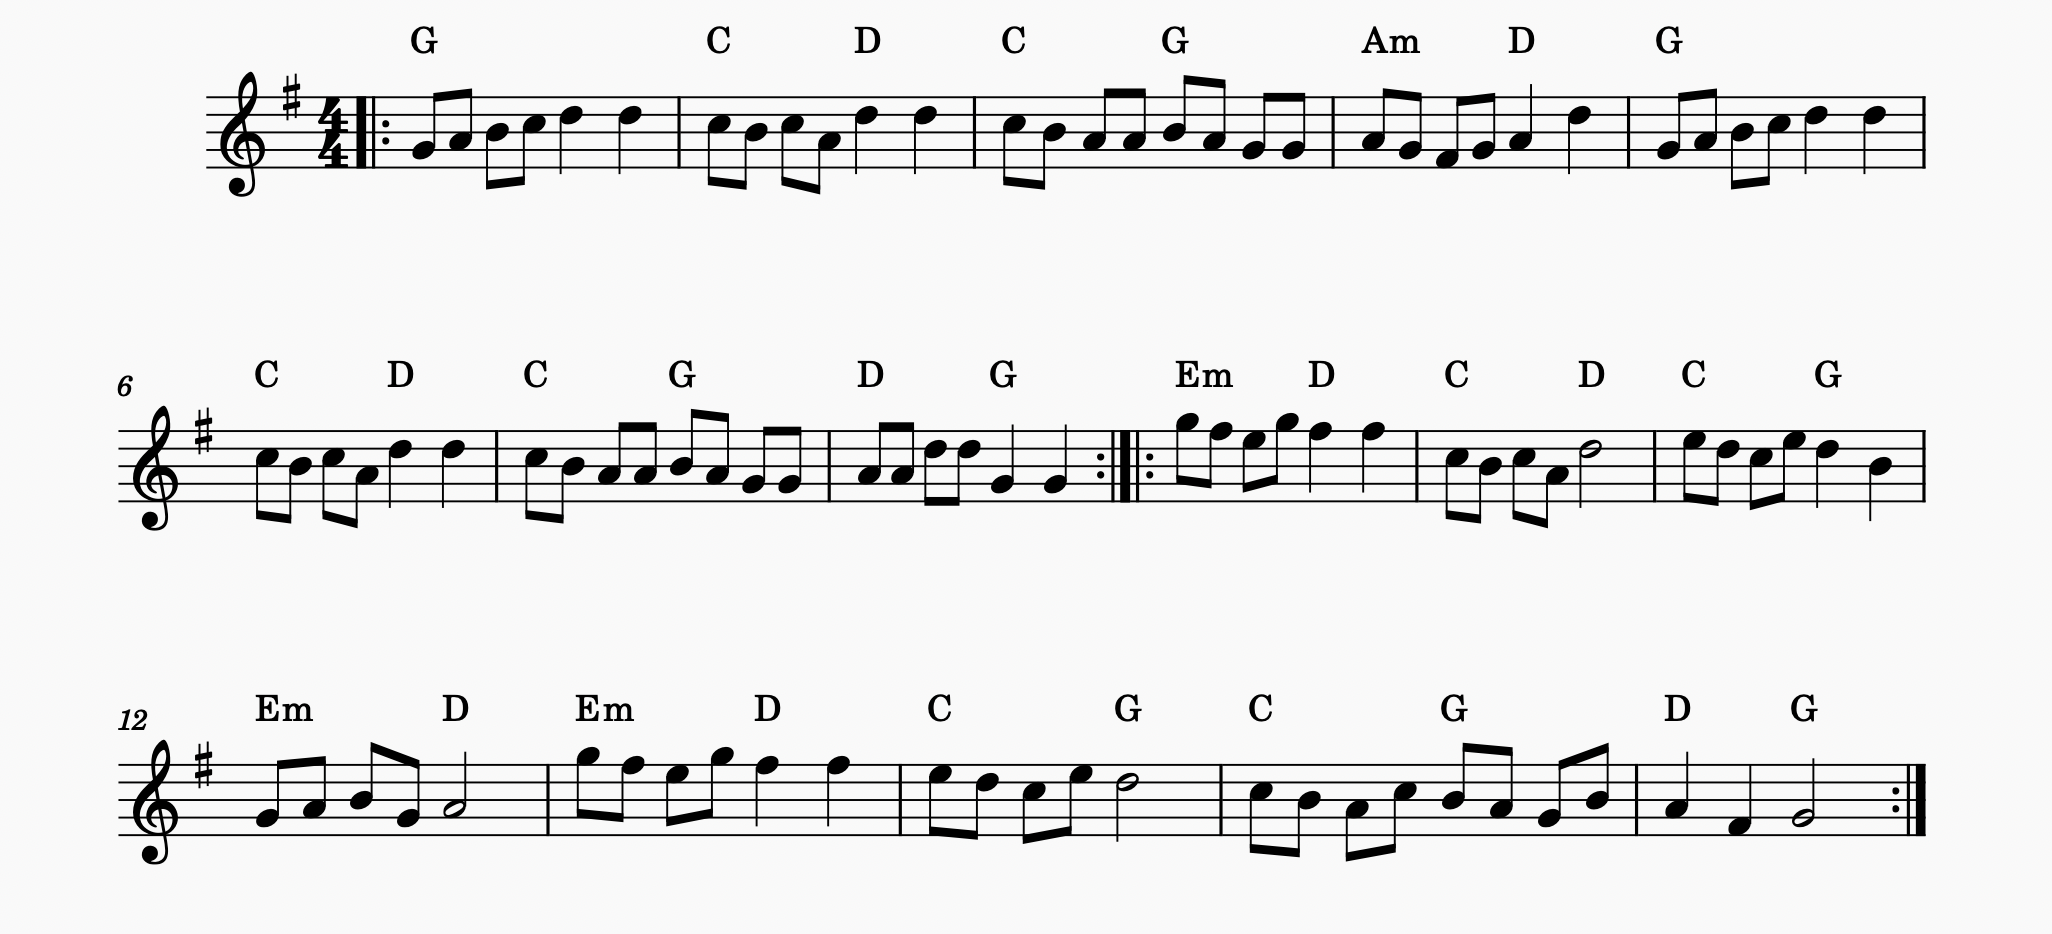
\includegraphics[width=\textwidth]{images/myscore.png}
    \caption{The standard musical score corresponding to the ABC notation provided in the example user prompt. This score is included for reference to help readers visualize the symbolic input.}
    \label{fig:myscore}
\end{figure*}

(1) We propose the first multi-agent symbolic music understanding system, M.U.S.E. It leverages the internal basic musical concept–understanding capabilities of LLMs without requiring external tools.

(2) Through the ABC-Eval benchmark\citep{zhaoABCEvalBenchmarkingLarge2025}, we demonstrate that our multi-agent solution improves symbolic music understanding compared with standalone LLMs. Since music composition requires LLMs to possess genuine musical understanding, the system’s enhanced capability could further advance research in music generation.

(3) Our method also provides cost-efficiency benefits by eliminating the need to retrain LLMs or deploy local inference services.

(4) We open-sourced our code to support progress in this research area and enable further exploration and development by the community.


\section{M.U.S.E.: Music Understanding System Engine}

\subsection{User prompt}
To demonstrate how our multi-agent framework interacts with end users, we provide an example prompt that a typical user might submit to the system. We intentionally choose a musically rich ABC score as the user input because it reflects a realistic use case in which a music lover or musician uploads symbolic music to learn what emotion the piece conveys. \autoref{fig:myscore} provides a standard score corresponding to this ABC notation for reference. The prompt below serves as a running illustration in the following section, where we explain the roles and responsibilities of each agent in the system.

\begin{tcolorbox}[
    title=Example of a user prompt, 
    colback=gray!10, 
    colframe=gray!60,
    before skip=2pt,   % <--- Add this to shrink the top space
    after skip=2pt     % <--- Good practice to keep bottom space balanced
    %listing only     % <--- DELETE THIS LINE (it conflicts with \textbf)
    ]
\textbf{ABC score:}
\begin{verbatim}
M:4/4
L:1/8
K:G
|:"G"GABc d2d2|"C"cBcA "D"d2d2|"C"cBAA "G"BAGG|
"Am"AGFG "D"A2d2|"G"GABc d2d2|"C"cBcA "D"d2d2|
"C"cBAA "G"BAGG|"D"AAdd "G"G2G2:|
|:"Em"gfeg "D"f2f2|"C"cBcA "D"d4|"C"edce "G"d2B2|
"Em"GABG "D"A4|"Em"gfeg "D"f2f2|"C"edce "G"d4|
"C"cBAc "G"BAGB|"D"A2F2 "G"G4:|
\end{verbatim}
\textbf{Question:} \\
What specific emotion does this music piece convey?
\end{tcolorbox}

\subsection{System Architecture}
We design our system as a modular multi-agent framework, shown in \autoref{fig:system}. This framework will interpret the user’s query about music scores in ABC notation and provide appropriate explanations to assist the user. Given the fact that users may completely miss or provide incomplete ABC music scores, the system first incorporates a Completion Detection Subsystem that performs completeness checks, contributing to the overall stability of the multi-agent system. 

The users will typically ask two major types of questions: (1) ABC syntax questions, which require the understanding of the symbolic representation of music and its structure. For example, the key, meter, rhythm, and chord functions of the music piece. (2) emotion-based questions, which require an understanding of music expression. The two major tasks require different forms of domain expertise and different views of the symbolic music representation, so we build two dedicated subsystems to handle them separately. 

The Controller Agent’s responsibility is to analyze the user’s query and determine whether the user’s question is about syntactical understanding, emotion-based, or a combination of both. It then decides which downstream subsystem to activate. If the Controller Agent identifies the user’s query as an ABC syntax question, it activates the Syntax Understanding Subsystem. This subsystem parses the ABC score, analyzes its structural representation, reasons about the symbolic music representation, and finally provides an answer to the user’s question. If the Controller Agent determines that the query is about emotion, the Emotion Understanding Subsystem is activated. This subsystem employs an arousal–valence framework for emotion classification: it first analyzes the arousal and valence levels of the ABC score separately, then uses an emotion-combiner agent to map these dimensions onto final emotion categories (Q1: happy, Q2: angry, Q3: sad, Q4: relaxed). It returns a structured answer with detailed reasoning for each dimension. 

The Aggregator agent is the last agent. It receives both answers from the Syntax Understanding Subsystem and the Emotion Understanding Subsystem and a decision from the Controller Agent. When the Controller identifies only one type of task, the Aggregator simply forwards the corresponding subsystem’s output.  When both ABC syntax and emotion-related questions are detected, the Aggregator will integrate the responses to produce a final answer for user.



\subsubsection{Completion Detection Subsystem}
The Completion Detection Subsystem operates before the Controller Agent. The role of this subsystem is to ensure that the user inputs a complete ABC notation with a question. Initially, we have a rule-based extraction script that can directly extract the ABC score if the user inputs the score in a standard format, such as code blocks, "Input:" or "Score:" markers, and ABC header fields (X:, K:, M:, L:). If this approach works, the Extraction Agent will be ignored, and the Inspector Agent will be activated. If the user's input is complex or does not follow the regular rules, the Extraction Agent will be activated. This hybrid approach combines the reliability of pattern matching with the flexibility of LLM-based extraction, ensuring robust input validation across a wide range of input formats, while keeping the calling minimal.

\begin{promptbox}{Example prompt of the Extraction Agent (when ABC score is not detected)}

You are an Extraction Agent for a music analysis system.\\

Your task is to check if the user input contains an ABC notation score.\\

User input:\\
\{user\_prompt\}\\

ABC notation typically:\\
- Starts with headers like X:, K:, M:, L:, R:\\
- Contains musical notes (A-G with optional sharps/flats and octaves)\\
- May be wrapped in code blocks (\texttt{``` ```}) or after "Input:" or "Score:"\\

Please analyze the user input and:\\
1. If you find ABC notation, extract it completely and respond with:\\
   EXTRACTED\_ABC:\\ 
   {[the complete ABC score here]}\\ 

2. If you confirm there is NO ABC notation, respond with:\\
   NO\_ABC\_SCORE\\

3. If the input is unclear or incomplete, respond with:\\
   UNCLEAR\_INPUT\\

Your response:
\end{promptbox}

\begin{promptbox}{Example prompt of the Inspector Agent (when ABC score is detected)}

You are an Inspector Agent for a music analysis system.\\

Your task is to:\\
1. Verify that the extracted ABC score is complete and correct\\
2. Check if the user has asked a question\\

User input:\\
\{user\_prompt\}\\

Extracted ABC score:\\
\{extracted\_abc\}\\

Please analyze and respond in one of these formats:\\

If the ABC score is complete and correct, AND the user has asked a question:\\
VALID\_INPUT\\

If the ABC score is incomplete or missing parts:\\
INCOMPLETE\_ABC:\\
{[description of what's missing or what should be added]}\\

If the user has NOT asked a question:\\
NO\_QUESTION\_DETECTED\\

If there are other issues:\\
ISSUE:\\
{[description of the issue]}\\

Your response:
\end{promptbox}

\subsubsection{Controller Agent}
The main responsibility of the Controller Agent is to understand the user’s query and pre-classify its type so that the system can maximize performance by activating the most suitable downstream subsystem. The Controller Agent outputs one of the following intent categories based on its analysis of the user’s query: ABC (if the query concerns ABC syntax), EMOTION (if the query concerns emotion-related questions), or BOTH (if the query involves both types).

\begin{promptbox}{Example prompt of the Controller Agent}
You are the Controller Agent.\\

Your job is to decide which specialized agents should be used.\\

Rules:\\
- If the user asks about ABC notation, keys, bars, chords -> respond "ABC"\\
- If the user asks about emotion, valence/arousal, mood -> respond "EMOTION"\\
- If both topics appear -> respond "BOTH"\\
- Otherwise -> respond "NONE"\\

Return ONLY ONE WORD.\\

User query:\\
\{user\_prompt\}\\
\end{promptbox}


\subsubsection{Syntax Understanding Subsystem}
This subsystem is activated when the Controller Agent determines that the user’s query concerns ABC syntax understanding. The Syntax Subsystem consists of two sub-agents: the ABC Score Expert Agent and the Evaluator Agent. 

The ABC Score Expert Agent is responsible for parsing the score and extracting structured musical information such as key, meter, note durations, and bar structure. It focuses solely on summarizing and organizing the musical content without attempting to reason about or answer the user’s question.

\begin{promptbox}{Example prompt of the ABC Score Expert Agent}

You are an ABC notation expert. Your job is to interpret the following ABC score.\\

Score:\\
\{input\_abc\}\\

Explain the meaning of each ABC component in a structured and concise way.\\
Focus on:\\
- Key (K:)\\
- Meter / time signature (M:)\\
- Default note length (L:)\\
- Chord symbols\\
- Bar boundaries\\
\\
Do NOT answer the user's question.\\
ONLY produce an analysis of the ABC score.\\
\end{promptbox}

The Evaluator Agent, in contrast, receives the analysis produced by the ABC Score Expert and uses it to answer the user’s music-theory questions.
This separation between parsing and reasoning improves both the stability and interpretability of the system. In the evaluation section, we compare this architecture with a single-LLM baseline and observe substantial performance improvements.

\begin{promptbox}{Example prompt of the Evaluator Agent}

You are the evaluator agent.\\

You will receive an analysis of an ABC score from the ABC Expert.\\
Your job is to answer the user's question based ONLY on that analysis.\\

ABC Expert Analysis:\\
\{analysis\}\\

Task:\\
\{user\_prompt\}\\

\end{promptbox}

\subsubsection{Emotion Understanding Subsystem}
This subsystem is activated when the Controller Agent determines that the user's query concerns emotion-related questions. The Emotion Understanding Subsystem has three sub-agents: the Arousal Analyst Agent, the Valence Analyst Agent, and the Emotion Combiner Agent. 

The Arousal Analyst Agent analyzes the provided ABC score and determines its arousal level (HIGH or LOW) based on musical features.

\begin{promptbox}{Example prompt of the Arousal Analyst Agent}

You are an Arousal Analyst Agent. Your job is to analyze the following ABC score and determine its arousal level.\\

Arousal classification:\\
- HIGH arousal: energetic, intense, driving\\
- LOW arousal: calm, peaceful, relaxed\\

Focus on observable musical features:\\
- Rhythmic density and tempo\\
- Motion continuity and activity\\
- Texture activity\\
- Pitch range and dynamics\\

Score:\\
\{input\_abc\}\\

Output format:\\
AROUSAL: <HIGH or LOW>\\
REASON: <brief explanation>\\

AROUSAL:
\end{promptbox}

Similarly, the Valence Analyst Agent analyzes the score to determine its valence level (HIGH or LOW). Each group contains three independent analysts to ensure robustness through majority voting. 

\begin{promptbox}{Example prompt of the Valence Analyst Agent}

You are a Valence Analyst Agent. Your job is to analyze the following ABC score and determine its valence level.\\

Valence classification:\\
- HIGH valence: pleasant, bright, joyful\\
- LOW valence: unpleasant, dark, sad\\

Focus on observable musical features:\\
- Harmonic quality and consonance\\
- Melodic contour and direction\\
- Key characteristics\\
- Overall emotional tone\\

Score:\\
\{input\_abc\}\\

Output format:\\
VALENCE: <HIGH or LOW>\\
REASON: <brief explanation>\\

VALENCE:
\end{promptbox}

Finally, the Emotion Combiner Agent receives the arousal and valence classifications produced by the respective analyst groups and determines the final emotion category (Q1–Q4, representing happy, angry, sad, and relaxed) according to the arousal–valence mapping.

\begin{promptbox}{Example prompt of the Emotion Combiner Agent}

You are the Emotion Combiner Agent.\\

You will receive arousal and valence classifications from the Analyst Agents.\\
Your job is to determine the final emotion category based on the arousal-valence mapping.\\

Categories:\\
0: Q1 (happy   - high valence, high arousal)\\
1: Q2 (angry   - low  valence, high arousal)\\
2: Q3 (sad     - low  valence, low  arousal)\\
3: Q4 (relaxed - high valence, low  arousal)\\

Mapping:\\
- High Valence + High Arousal → Label 0\\
- Low Valence + High Arousal → Label 1\\
- Low Valence + Low Arousal → Label 2\\
- High Valence + Low Arousal → Label 3\\

Score:\\
\{input\_abc\}\\

Arousal Analysis:\\
\{arousal\_result\}\\

Valence Analysis:\\
\{valence\_result\}\\

Answer:
\end{promptbox}
This structure can increase the stability and interpretability of classifying musical emotion by separating the dimensional analysis from the final classification. In addition, this independence will make their analysis more objective. In the evaluation section, we compare this subsystem with a single LLM baseline and observe significant performance improvements.

\subsubsection{Aggregator Agent}
The Aggregator Agent is responsible for producing the final answer to the user’s query. 
If the Controller Agent’s decision is ABC, the Aggregator Agent returns only the output from the Syntax Understanding Subsystem.
If the decision is EMOTION, it returns only the output from the Emotion Understanding Subsystem.
If the decision is BOTH, the Aggregator Agent receives answers from both subsystems, merges the outputs from both subsystems, and provides an integrated response to the user.

\begin{promptbox}{The Aggregation logic}
Check the controller's decision. \\ 

If the decision is ABC:\\
    Return only Agent B's output.\\

If the decision is EMOTION:\\
    Return only Agent C's output.\\

If BOTH:\\
    Return both outputs, merged in order.\\
\end{promptbox}

\subsection{Advantage}
Overall, we designed a multi-agent architecture in which each subsystem handles a specific music understanding task, allowing the system to optimize its solution based on the most appropriate prompt template and internal reasoning process designed for each sub-task. This modular structure has three advantages. First, it provides strong interpretability, as the behavior of each module is transparent and traceable. Second, the modular architecture makes it easy to add additional functional subsystems without modifying existing modules, such as a harmony agent or a music generation agent. Third, when a user’s query involves multiple aspects. For example, first asking about the structure of the music score and then the emotional color it conveys, the multi-agent architecture can invoke the corresponding experts separately and then use another agent to aggregate and integrate their outputs into a coherent answer, avoiding the confusion or hallucination that may occur when a single large model performs cross-domain reasoning.

\section{Experiment}
\subsection{Setup}
\subsubsection{Benchmark}
A major difficulty in symbolic music understanding is verifying whether a model truly understands the symbolic music structure, rather than producing plausible but hallucinated answers. Unlike other music AI tasks, such as genre classification based on audio perception or evaluating creative outputs where judgment often relies on human listening and subjective scoring, symbolic music understanding demands more objective, quantitative, and fine-grained benchmarks. This is essential for helping us distinguish the structural reasoning from surface-level pattern matching. 

To address this need, we draw inspiration from the recent \citet{zhaoABCEvalBenchmarkingLarge2025}, which combines several symbolic-music datasets into well-defined multiple-choice and numeric prediction tasks. These tasks are designed to test specific aspects of music understanding in a measurable and objective way. The benchmark decomposes symbolic music reasoning into three major categories: Basic Syntax Understanding (e.g., Bar Count Estimation, Metadata Q\&A); Segment-level Understanding(e.g., Bar Sequencing, error detection); Sequence-level Understanding (e.g., Emotion Recognition). Each category assesses different aspects of symbolic music understanding, ranging from low-level information extraction from symbolic music scores to high-level semantic interpretation, such as describing the emotion of the provided symbolic music score. With this benchmark, it is possible to meaningfully compare the behavior of pure LLMs and agentic systems without stepping into subjective evaluation or open-ended outputs. In our experiments, we select two representative tasks from the ABC-EVAL benchmark: Metadata Q\&A and Emotion Recognition. The detailed information is in \autoref{tab:tasks}. 

We choose these tasks for two main reasons. First, they capture two levels of symbolic music understanding. Metadata Q\&A focuses on low-level syntactic reasoning, such as key, meter, and bar structure, which allows us to evaluate whether the model truly understands the symbolic meaning of ABC notation and its ability to parse symbolic notation correctly. In contrast, Emotion Recognition requires higher-level semantic interpretation that relies on melodies, chord progressions, rhythmic cues, and etc. These tasks provide a balanced view of both structural and semantic understanding. 

\begin{table}[H]
\centering
\begin{tabular}{lcc}
\toprule
\textbf{Task} & \textbf{Category} & \textbf{Size} \\
\midrule
\textbf{Metadata Q\&A} & Basic Syntax & 60 \\
\textbf{Emotion Recognition} & Sequence-Level & 100 \\
\bottomrule
\end{tabular}
\caption{Subset of evaluation tasks used in our study.}
\label{tab:tasks}
\end{table}

\subsubsection {Evaluation Protocol}
For benchmarking purposes, we directly invoke the subsystem responsible for each task rather than routing queries through the Controller Agent. This allows us to isolate and evaluate the symbolic-music understanding capabilities of each specialized subsystem without confounding the results with routing errors. Our goal is to measure the musical reasoning performance of the subsystems and the performance of key agents, rather than the orchestration mechanism. To evaluate the subsystems, we took two tasks from the ABC-Eval benchmark: Metadata Q\&A questions and Emotion Recognition questions. Metadata Q\&A questions mainly focus on the basic syntax understanding of music score in ABC notation. For example, in Metadata Q\&A, the multiple choice question might ask the key signature of the music piece or the time signature of the music piece. Among all four choices, there is only one correct answer. 

\begin{tcolorbox}[title=Metadata Q\&A, colback=gray!10, colframe=gray!60, listing only]
\begin{verbatim}
M:4/4
L:1/8
K:G
|:"G"GABc d2d2|"C"cBcA "D"d2d2|"C"cBAA "G"BAGG|
"Am"AGFG "D"A2d2|"G"GABc d2d2|"C"cBcA "D"d2d2|
"C"cBAA "G"BAGG|"D"AAdd "G"G2G2:|
|:"Em"gfeg "D"f2f2|"C"cBcA "D"d4|"C"edce "G"d2B2|
"Em"GABG "D"A4|"Em"gfeg "D"f2f2|"C"edce "G"d4|
"C"cBAc "G"BAGB|"D"A2F2 "G"G4:|

Task:
Identify the time signature of the provided 
ABC notation score.

Options:
0. 4/4   1. 3/4
2. 6/4   3. 6/8
\end{verbatim}
\end{tcolorbox}

The Emotion Recognition task, on the other hand, focus on sequence-level understanding of music score in ABC notation. Similar to Metadata Q\&A, it provides a ABC score and 4 choices of emotion label and there is only one correct answer.

\begin{tcolorbox}[title=Emotion Recognition, colback=gray!10, colframe=gray!60, listing only]
\begin{verbatim}
M:4/4
L:1/8
K:G
|:"G"GABc d2d2|"C"cBcA "D"d2d2|"C"cBAA "G"BAGG|
"Am"AGFG "D"A2d2|"G"GABc d2d2|"C"cBcA "D"d2d2|
"C"cBAA "G"BAGG|"D"AAdd "G"G2G2:|
|:"Em"gfeg "D"f2f2|"C"cBcA "D"d4|"C"edce "G"d2B2|
"Em"GABG "D"A4|"Em"gfeg "D"f2f2|"C"edce "G"d4|
"C"cBAc "G"BAGB|"D"A2F2 "G"G4:|

Task:
Choose the most probable emotional label of the 
provided score. 
Label Q1 refers to happy (high valence high arousal), 
Q2 refers to angry (low valence high arousal), 
Q3 refers to sad (low valence low arousal) and 
Q4 refers to relaxed (high valence low arousal).

Options:
0. Q1      1. Q2
2. Q3      3. Q4
\end{verbatim}
\end{tcolorbox}

To evaluate the performance of the Controller Agent, we randomly generate ABC notation data and present it with 1-3 questions. These questions assess syntax understanding (such as counting bars or identifying the key signature), evaluate emotion (for example, identifying the emotion), or address both aspects. We then test whether the Controller Agent correctly classifies each question type.

\subsection{Evaluation}
We evaluate two baseline LLMs: google/gemma-3-27b-it and meta-llama/Meta-Llama-3.1-70B-Instruct.
Two models have different performance in our study, and we include both of them to examine whether our agentic framework can compensate for the limited model's capacity. By comparing these two models in both standalone and agentic settings, we assess two things: 1. their individual symbolic-music reasoning ability. 2. The extent to which our multi-agent system amplifies the strengths or mitigates the weaknesses of the underlying LLMs.

\subsubsection{Controller Performance}
Based on our test on 100 randomly generated samples, both Meta LLaMA and Google Gemma could classify all the users' questions correctly (accuracy rate 100\%). This ensures the test on the subsystem is a reasonable proxy of the whole agent.

\subsubsection{Standalone Performance}
Based on \autoref{tab:llm-agent-compare}, we can see the performance of standalone LLMs on symbolic music understanding tasks. Meta LLaMA demonstrates low performance on both the Metadata Q\&A tasks and the Emotion Recognition tasks, while Google Gemma performs well on the Metadata Q\&A tasks and shows much better performance on the Emotion Recognition tasks, though still not ideal. We can see that current LLMs still struggle to understand symbolic music in ABC notation and can only weakly reason about it, leaving plenty of room for improvement for an agentic solution.

\begin{table}[H]
\centering
\resizebox{\linewidth}{!}{%
\begin{tabular}{p{3cm} *{4}{c}}
\toprule
\textbf{Task} &
\multicolumn{2}{c}{\textbf{Meta-Llama-3.1-70B-Instruct}} &
\multicolumn{2}{c}{\textbf{gemma-3-27b-it}} \\
\cmidrule(lr){2-3}\cmidrule(lr){4-5}
& \textbf{LLM} & \textbf{Agent} & \textbf{LLM} & \textbf{Agent} \\
\midrule
\textbf{Controller} & not apply\ & \textbf{100\%} & not apply\ & \textbf{100\%} \\
\textbf{Metadata Q\&A} & 61.67\% & \textbf{98.33\%} & \textbf{98.33\%} & \textbf{98.33\%} \\
\textbf{Emotion Recognition} & 14.00\% & 38.00\% & 18.00\% & \textbf{53.30\%} \\
\textbf{- Arousal} & 38.00\% & 60.00\% & 34.00\% & \textbf{76.67\%} \\
\textbf{- Valence} & 40.00\% & 58.00\% & 59.00\% & \textbf{60.00\%} \\
\bottomrule
\end{tabular}
}
\caption{Comparison of standalone LLM accuracy vs. agentic performance on two ABC-Eval tasks.}
\label{tab:llm-agent-compare}
\end{table}

\subsubsection{Agentic Performance}
For the evaluation of the multi-agent system, we first test the Controller Agent and find that, for both the LLaMA and Gemma, it classifies the question type into the correct category on our queries for all of the test questions. This makes evaluating the task-specific subsystems a reasonable proxy for the performance of the full agentic system.

We then test the performance of our agentic solution. Specifically, we evaluate the Metadata Q\&A questions using our Syntax Understanding Subsystem and the Emotion Recognition questions using our Emotion Understanding Subsystem. For the Metadata Q\&A task, we observe a drastic increase in performance when building the agent framework on top of Meta LLaMA, from 61.67\% to 98.33\%, and consistently strong performance when building on top of Google Gemma, both achieving 98.33\%. These results highlight an important effect of the agent architecture: We effectively reduce the reasoning burden on the underlying LLM. Even a small model like Meta LLaMA, which performs poorly when asked to interpret ABC notation directly, can achieve nearly perfect accuracy with our agentic solution. This suggests that the agentic approach does not merely improve accuracy, but  changes the nature of the task, allowing weaker model can be a reliable option to solve the questions.

For the Emotion Recognition task, the problem is substantially more challenging, and the agentic system provides more significant improvement. When directly asked to choose among the four discrete emotion labels, one-shot LLM achieve 14.00\% and 18.00\% accuracy for Meta LLaMA and Google Gemma. The result is worse than random guessing, which have the expected accuracy of 25\%. With the Emotion Understanding Subsystem, the accuracy improved to 38.00\% for Meta LLaMA and 53.30\% for Google Gemma. While the absolute accuracy still have room for improvement, the relative gains are considerable. This indicates that decomposing the understanding problem into a structured pipeline, where the high or low of the arousal and valence are separately determined first, and then the categorical labels are mapped based on the previous analysis, helps the model make a better understanding of the musical emotion. If we look into the details of the emotion recognition, we also observe that the improvement on the arousal component is particularly pronounced. This suggests that, when an LLM is directly asked to judge the overall emotion, its arousal judgment is more easily influenced by irrelevant textual or contextual factors, whereas explicitly factoring out arousal as an intermediate step within the agentic pipeline leads to more stable and robust predictions.

\section{Discussion}
Our research results indicate that applying a multi-agent system to symbolic music understanding has both potential and limitations. 

In metadata Q\&A tasks, our agent-based solutions nearly eliminate the performance gap between weaker and stronger language models. While the baseline model LLaMA has an accuracy far below that of Gemma, after introducing a Syntax Understanding Subsystem, the performance of the two models is almost identical, with both correctly answering 59 out of 60 questions. This suggests that the bottleneck for the weaker model is not merely a lack of musical knowledge, but the difficulty of doing score information parsing and reasoning the question at the same time. By explicitly separating these stages, our agentic solution M.U.S.E. reformulates the problem into a more manageable form: an ABC Score Expert Agent first performs a structured analysis of the score, and then an Evaluation Agent reasons and provides solutions based solely on this analysis. This division of work reduces the reasoning burden on the underlying model and makes the model's behavior more stable and interpretable.

Similarly, in the emotion recognition task, the problem is much more challenging. Both Meta LLaMA and Gemma perform poorly when they are required to directly choose among four discrete emotion labels. In that case, the accuracy is close to or even below random guessing. After introducing the Emotion Understanding Subsystem, the performance improves remarkably for both Meta LLaMA and Gemma. The key factor is that the subsystem decomposes the emotion recognition task into dimensional judgement and a simple mapping. Specifically, we break direct emotion recognition into valence analysis and arousal analysis, where valence and arousal are two dimensions, and when combined together, they can describe a certain emotion. With this implementation, our Arousal Analyst Agent and Valence Analyst Agent first decide on HIGH/LOW arousal and valence, and the Emotion Combiner Agent then maps this two-dimensional representation to an emotion label in multiple-choice questions. The fact that this pipeline provides a large accuracy boost indicates that LLMs find it easier to reason in an individual arousal or valence level and provide local justifications than to directly commit to an emotion category label. In other words, the agent system changes the structure of the problem in a way that better aligns with how LLMs process symbolic music information.

However, our system is far from solving symbolic music understanding. Emotion Recognition accuracy remains well below ceiling even with the Emotion Understanding Subsystem, and the arousal and valence sub-tasks themselves are still noisy. We also observe that improvements on the arousal dimension are generally more pronounced than on valence. This is plausible that arousal is strongly associated with rhythmic density, motion, and surface-level activity patterns that are relatively easy to infer from ABC notation, whereas valence depends more on harmonic context, modality, and longer-range melodic tendencies, which are more subtle and harder to capture from symbolic input alone. These results suggest that purely symbolic cues, while useful, do not fully account for the perceived emotion of a piece, and that additional information (such as expressive performance features) may be needed for more accurate affective modeling.  

It is also important to note that musical emotion is inherently subjective. The four-quadrant labels in our benchmark ultimately originate from human annotations, so the “ground-truth” emotion for a given piece somewhat relies on human judgments rather than an objective property of the score. As a result, some predictions that are counted as errors by our metrics are musically reasonable alternatives. In a small-scale manual re-check on a subset of items where the model’s output disagreed with the provided label, members of our team occasionally judged the model’s label to be a plausible interpretation of the music. However, this analysis is based on limited internal sampling and cannot be taken as evidence that the benchmark label is wrong or that our preferred label reflects the true emotion. 

In future work, we plan to refine the dataset through more systematic human studies, collecting distributions over emotion labels instead of single hard assignments. Such soft-label annotations would help identify inherently ambiguous pieces, provide a more faithful estimate of model performance, and provide a better basis for improving emotion-aware symbolic music models and, ultimately, guiding symbolic music generation.

\section{Conclusion}
Considering the limited ability of large language models (LLMs) to understand symbolic music and the shortcomings of current music-related agent systems, we built M.U.S.E. - a multi-agent system designed to enhance symbolic music understanding with LLMs without relying on external music-processing tools. By evaluating performance on both syntax understanding and emotion recognition tasks, we demonstrate that our multi-agent system can perform better than single LLMs alone.  Our agentic solution also highlights several directions for future development, including the possibility of incorporating additional music understanding tasks beyond our current two representative tasks, such as harmony analysis, bar sequencing, and genre detection. Overall, our experimental results show that a multi-agent system is effective for symbolic music understanding and offers a pathway for bridging music knowledge and music reasoning in current LLMs.

\section*{Contribution}
\textbf{Core}\\
Chenxi Peng chenxipeng@uchicago.edu\\
Chenqi Wang chenqiw@uchicago.edu\\
Qicheng Jin qjin5@uchicago.edu\\

\section*{Github Repo for our project}
https://github.com/chenqiww/muse-Multi-agent-Symbolic-Music-Understanding/tree/main

\section*{Dataset Sources}

\noindent\textbf{ABC/Metadata QA and Emotion Recognition Dataset:}\\
ABC-Eval: A Comprehensive Benchmark for Evaluating Large Language Models
on ABC Notation Understanding.\\
\url{https://anonymous.4open.science/r/ABC-Eval-B622}

\medskip

\noindent\textbf{Emotion Recognition Dataset:}\\
Zhou, M., Li, X., Yu, F., \& Li, W. (2023).\\
EMelodyGen: Emotion-Conditioned Melody Generation in ABC Notation.\\
\url{https://arxiv.org/abs/2309.13259}\\
Dataset: \url{https://huggingface.co/datasets/monetjoe/EMelodyGen}

% ----------------------------------------------------------------------
% Bibliography
% ----------------------------------------------------------------------
\bibliographystyle{ACM-Reference-Format}
\bibliography{references}



\end{document}
